
\chapter{Аналитический раздел}

В данном разделе будут представлены обзор предметной области, существующих методов определения позы человека, а также проведен сравнительный анализ этих методов.

\section{Обзор предметной области}

\subsection{Классические подходы к определению позы человека}

Глубокое обучение --- тип машинного обучения \cite{vyugin}, в котором используются искусственные нейронные сети с несколькими слоями для обработки сложных данных, которые активно используются в настоящее время в определении позы человека. Однако до его внедрения использовались другие методы, а именно: 
\begin{enumerate}[label=\arabic*)]
 	\item Модель пиктографических структур \cite{polygraphic}:
 	
 		Эта структура моделирует пространственные взаимосвязи частей твердого тела, выражая их в виде древовидной графической модели, чтобы предсказать местоположение суставов тела. 
 		Эти пространственные связи показаны с помощью пружин, и части представляют собой шаблоны внешнего вида, основанные на изображении. 
 		Путем параметризации частей с помощью расположения и ориентации пикселей, полученная структура может моделировать артикуляции. 
 		
 		На рисунке \ref{img:polygraphic} продемонстрировано наглядное представление этой модели.
 		
 		Проблема этого подхода заключается в том, что он не может уловить корреляции между невидимыми и деформируемыми частями тела, что означает, что модель подвержена ошибкам, если не все конечности человека видны. 
 		Она также не зависит от данных изображения.
 		\begin{figure}[ht!]
 			\centering
 			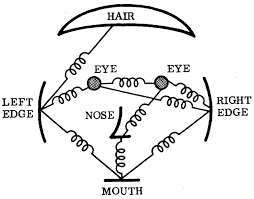
\includegraphics[width=0.4\linewidth]{assets/poly.png}
 			\caption{Пример пиктографической структуры.}
 			\label{img:polygraphic}
 		\end{figure}
 		

 	\item Гибкое смешение частей \cite{FPE}:
 		
 		\begin{itemize}
 			\item Этот подход использует деформируемые модели частей, которые представляют собой коллекцию шаблонов, которые подбираются по изображению и располагаются в деформируемой конфигурации. 
 			Кроме того, каждая модель имеет глобальные шаблоны и шаблоны деталей. 
 			Основная идея заключается в том, чтобы использовать смесь мелких неориентированных деталей в отличие от использования семейства деформированных, то есть повернутых и ракурсных шаблонов.
 			Причина этого заключается в том, что с различиями в том, как выглядят конечности, и изменениями в точке зрения.
 			
 			\item Гибкое смещение частей одновременно фиксирует пространственные отношения между расположением деталей и отношения совпадения между смесями деталей, что приводит к моделям пиктографического структуры, которые кодируют исключительно пространственные отношения. 
 			Благодаря динамическому программированию, модели разделяют вычисления между аналогичными искривлениями, что делает этот подход не только значительно быстрым, но и высокоэффективным.
 			Кроме того они моделируют экспоненциально большой набор глобальных смесей через композицию смесей локальных частей для того, чтобы изучить понятия локальной жесткости, а также уловить влияние глобальной геометрии на локальный внешний вид, то есть внешний вид деталей различается в разных местах. 
 			На рисунке \ref{img:fpe} демонстрируется визуальное представление этой модели.
 			
 			\begin{figure}[ht!]
 				\centering
 				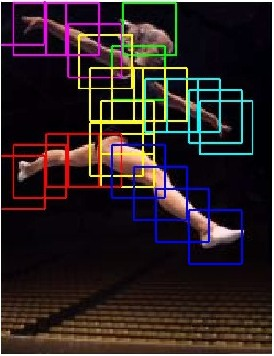
\includegraphics[width=0.4\linewidth]{assets/fpe.jpeg}
 				\caption{Пример гибкого смещения частей.}
 				\label{img:fpe}
 			\end{figure}
 			
 			\item Гибкое смещение частей способна хорошо выражать сложные отношения между суставами, поэтому она также может моделировать артикуляцию.
 			Однако у нее есть свои проблемы, которые включат ограниченную выразительность и отсутствие учета глобального контекста.
 			
 				
 		\end{itemize}
 		
 		
 	\item Края, цветочные гистограммы, контуры и гистограмма ориентированных градиентов были другими характеристиками, которые применялись в ранних работах определения позы человека и служили основными строительными блоками различных классических моделей для определения точного местоположения частей тела \cite{polygraphic}. 
\end{enumerate}

К общим проблемам классических подходов относятся плохое обобщение и неточное обнаружение частей тела. Поэтому для решения этих проблем было применено глубокое обучение.

\section{Глубокое обучение в сверточных нейронных сетях в машине позирования}

Машина позирования состоит из последовательных мультиклассовых предсказаний, которых обучены предсказывать местоположение каждой детали на каждом уровне иерархии. Она также имеет модуль вычисления характеристик изображения и модуль предсказания, оба из которых могут быть заменены сверточной архитектурой \cite{CNN}, что позволяет позволяет изучать как изображения, так и контекстуальные представления признаков из данных.
Именно эта идея привела к созданию Convolutional Pose Machine (CPM), которая является первой моделью оценки позы человека на основе глубокого обучения \cite{wei2016cpm}.

CPM полностью дифференцируема, что позволяет обучать ее многоступенчатую архитектуру по принципу обратного распространения, алгоритму, используемому для обучения нейронных сетей с прямой передачей 
Кроме того, ее последовательная структура предсказания, состоящая из сверточных сетей и обучается неявным пространственным моделям, использует большие рецепторные поля на картах убеждений, полученных на предыдущих этапах, что помогает в изучении пространственных связей между деталями на большом расстоянии и приводит к повышению точности за счет все более точных оценок местоположения деталей на последующих шагах.

Проблема исчезающих градиентов, когда при обратном распространении ошибки, градиенты уменьшаются по мере прохождения через многие слои решается с помощью промежуточного контроля после каждого этапа \cite{wei2016cpm}.

На первом этапе CPM предсказывает предположения о деталях, используя только локальные данные изображения, с помощью глубокой сверточной сети, состоящей из 7 общих сверточных слоев. Карты убеждений, созданные на этом этапе, добавляются к вводимым данным перед обработкой несколькими сверточными слоями.

На более поздних этапах эффективное восприимчивое поле увеличивается для повышения точности. 
В целом, этот подход позволяет архитектуре изучать как особенности изображения, так и пространственные модели, зависящие от изображения, для задач прогнозирования без необходимости использовать графический стиль моделирования выводы.

На рисунке \ref{img:cpm} показан пример работы CPM.
\begin{figure}[ht!]
	\centering
	\includegraphics[width=1\linewidth]{assets/cpm.png}
	\caption{Пример работы CPM.}
	\label{img:cpm}
\end{figure}

\section{Точность и метрики}

\subsection{Определение точности и понятие метрики}

Определение точности --- это оценка машинного обучения путем вычисления показателей их алгоритмов \cite{vyugin}. 
Существует множество оценочных метрик. используемых для проведения таких вычислений.
Причина этого заключается в том, что существует множество характеристик и требований, которые необходимо учитывать при оценке показателей модели оценки позы человека.
Таким образом, другими словами, точность модели определяется с помощью метрик, то есть метрики --- это способ количественной оценки точности модели.

\subsection{Различные метрики, используемые в определении позы человека}

Как было сказано ранее, существует несколько метрик, используемых для оценки эффективности моделей определения поз человека.

Ниже перечислены некоторые из них:

\begin{enumerate}[label=\arabic*)]
	
	\item Пересечение над объединением (ПНО) \cite{IoU}: это метрика, которая находит разницу между истинными и предсказанными ограничительными рамками.
	Удаляет все ненужные на основе установленного порогового значения, которое обычно составляет 0,5.
	
	\item Процент правильных частей (ППЧ) и Процент обнаруженных соединений (ПОС) \cite{PDJ}: это метрика, которая сейчас не так часто используется, но ее цель заключалась в том, чтобы сообщить о точности локализации конечностей.
	Это определяется, когда расстояние между предсказанными и истинными суставами меньше, чем доля длины конечности, которая составляет от 0,1 и 0,5.
	Если порог равен 0,5, то показатель ППЧ называется ППЧ@0,5.
	Более высокий показатель ППЧ означает лучшую производительность
	Ограничение этой метрики, в тоже время заключается в том, что она является неточной для конечностей с небольшой длинной.
	В связи с этим был внедрен ПОС, который следует той же логике, что и ППЧ; если расстояние между предсказанным и истинным суставами находится в пределах опредленной доли диаметра туловища, сустав считается правильно обнаруженным.
	Использование этой метрики подразумевает, что точность определения всех суставов основывается на этом пороге.
	
	\item Процент правильных ключевых точек  (ППКТ) \cite{guide-hpe}: эта метрика используется для измерения точности локализации различных ключевых точек в пределах опредленного порога.
	Он установлен на 50\% от длины сегмента головы каждого тестового изображения.
	Связано с ПОС, когда расстояние между обнаруженными и истинными суставами меньше, чем 0,2 диаметра туловища, это называется ППКТ@0,2.
	Чем выше значение ППКТ, тем лучше показатели.
	
	\item Средняя точность (СТ) \cite{guide-hpe}: СТ измеряет точность обнаружения ключевых точек в соответствии с точностью, которая представляет собой отношение истинно положительных результатов к общему количеству положительных результатов.
	Другими словами, насколько точным являются предсказания. 
	Таким образом, метрика СТ представляет собой среднее значение точности по всем значениям отзыва от 0 до 1 при различных пороговых значений ПНО.
	
	\item Средневзвешенная точность (СТ) \cite{guide-hpe} --- это среднее значение средней точности по всех классов при различных пороговых значениях ПНО по всей модели.
	
\end{enumerate}
